\section{Introduction}
\label{sec:introduction}
%%%%%%%%%%%%% 我们干了啥事 %%%%%%%%%%%%
% 1.在 few-shot SPR 上对 generic/surgical FM 做了简单对比，发现 generic FM（DINOv3）潜力很大
% 2.选择DINOv3作为generic FM，然后针对性设计了video适配的策略
% 3.考虑临床部署挑战，提出了异构蒸馏策略
% 4.我们实验丰富，public和private数据集都验证few-shot优势明显，实时性部分也极大提升

% 总结三大卖点：generic FM 适配、few-shot即可高acc、计算效率实时性轻量化
%%%%%%%%%%%%%%%%%%%%%%%%%%%%%%%%%%%%%%%%%%%%%


\IEEEPARstart{S}{urgical} phase recognition (SPR), which identifies frame-wise surgical intentions from procedural videos, is foundational for intelligent operating rooms by supporting intraoperative decision support~\cite{vermeulen2023ultra}, real-time anomaly detection~\cite{mithany2023advancements}, and postoperative skill assessment~\cite{cao2023intelligent}. 
Recently, the domain has shifted toward pre-training surgical foundation models (FMs) on expansive corpora~\cite{batic2024endovit,yang2026large,wu2026surgmotion}, demonstrating promising performance. 
However, this relentless scaling introduces key clinical barriers that remain under-addressed. On one hand, curating massive surgical datasets incurs prohibitive annotation costs, privacy risks, and procedural biases. On the other hand, the associated parameter explosion renders heavy architectures computationally infeasible for resource-constrained clinical hardware. Crucially, practical SPR demands real-time inference, as instant intraoperative feedback directly impacts patient safety. Consequently, amid the push for larger surgical FMs, simultaneously overcoming heavy data reliance and deployment latency remains a critical yet overlooked challenge for practical SPR.

To address the data burden, general visual FMs offer a promising avenue by leveraging rich pretrained representations for downstream adaptation under limited supervision. Generic FMs have evolved rapidly across image and video domains, spanning self-supervised frameworks such as DINOv3~\cite{simeoni2025dinov3} and VideoMAEv2~\cite{wang2023videomae} alongside vision-language contrastive models like CLIP~\cite{radford2021learning} and InternVideo2~\cite{wang2024internvideo2}. Intriguingly, our systematic evaluation across five surgical datasets reveals that generic FMs match or outperform specialized surgical FMs in few-shot scenarios, despite lacking surgical pretraining exposure. Motivated by this observation, we select DINOv3 as the backbone and propose DINO-SPR, a novel spatiotemporal adaptation framework for few-shot settings. By incorporating salient spatial token selection (SSTS) and keyframe-prior temporal fusion (KPTF), DINO-SPR filters irrelevant background while preserving discriminative moments for effective video understanding. Consequently, with only a handful of labeled videos, this adaptation unlocks the strong potential of generic FMs for SPR without relying on massive surgical corpora.

Although DINO-SPR demonstrates remarkable data efficiency, its reliance on a heavy ViT backbone introduces heavy computational overhead and rigid deployment constraints. To overcome this bottleneck, we propose an architecture-agnostic distillation strategy that transfers the teacher into DINO-SPR Lite. To bridge the teacher-student structural discrepancy, a cross-attention projection (CAP) maps heterogeneous student feature maps into the teacher's token space, enabling flexible supervision across CNN, ViT, and hybrid architectures. Complementing this alignment, a spatiotemporally-guided distillation (STGD) transfers spatial and temporal priors into intermediate student representations, supplying the dense supervisory signals missing under scarce annotations. As shown in Fig.~\ref{fig:tradeoff}, the resulting DINO-SPR Lite models across three diverse student families achieve real-time CPU inference while approaching teacher-level accuracy, successfully reconciling accuracy and speed for clinical deployment.


\begin{figure}[t]
\centerline{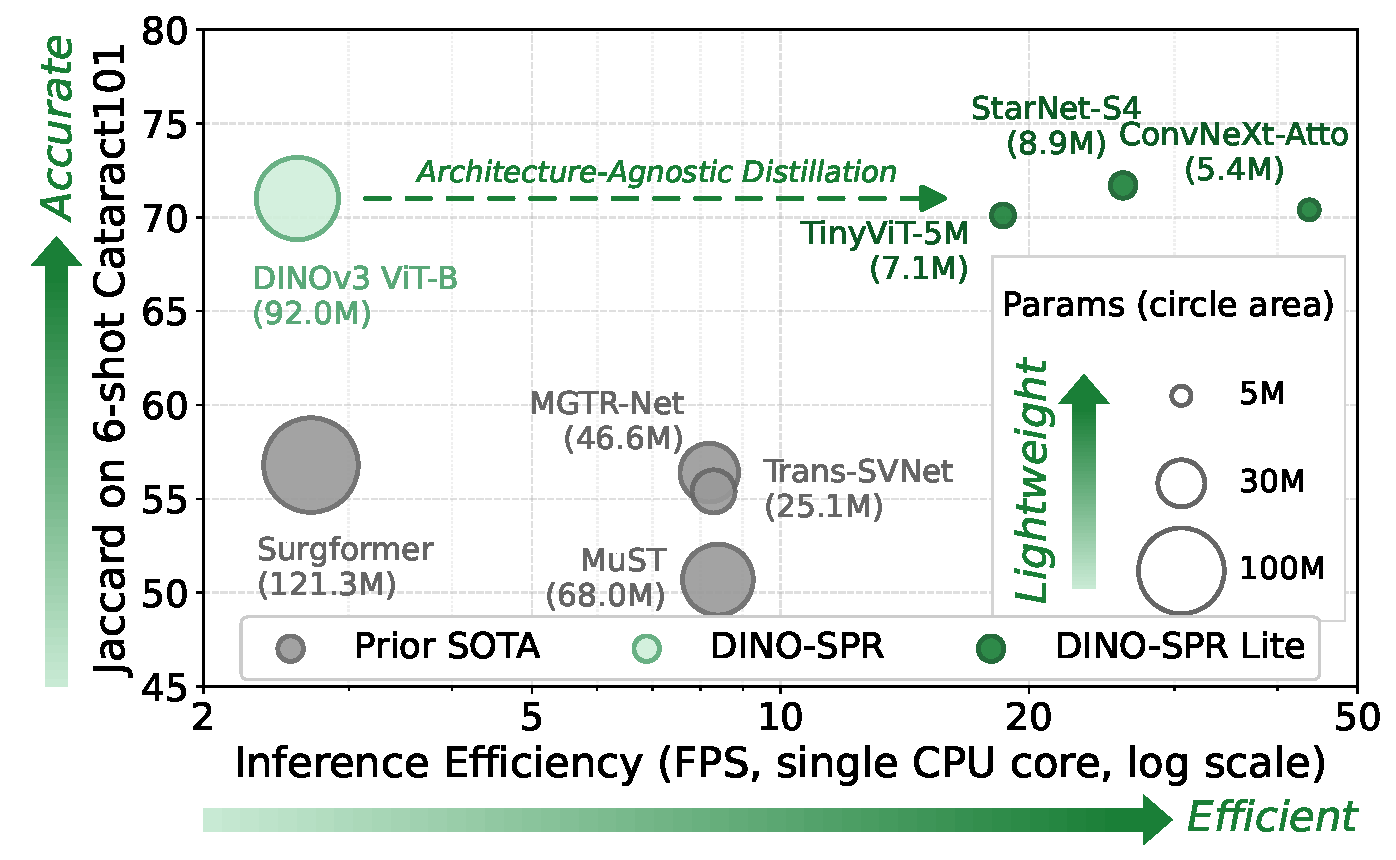
\includegraphics[width=\columnwidth]{resources/fig_computational_cost.pdf}}
\caption{6-shot Cataract101 Jaccard against inference efficiency on CPU, with circle area proportional to parameter count. Prior methods (gray) stay below 8.4\,FPS, while the DINO-SPR Lite students (dark green) match the DINO-SPR teacher (light green) at 18.6 to 43.7\,FPS.}
\label{fig:tradeoff}
\end{figure}


Our contributions could be summarized as follow:
% 贡献1：在 few-shot SPR 上对 representative 的 generic/surgical FM 做了简单对比，发现 generic FM DINOv3 的 few-shot 泛化潜力很大，由此选定 backbone
% 我们设计了video adaptation的策略，把image-based的DINOv3模型快速适配到surgical video任务
% 我们提出了异构模型蒸馏的方法，将few-shot适配后的DINOv3蒸馏到不同架构的轻量化模型，极大地提升了临床部署效率
% 5个手术阶段识别数据集，其中包含一个私有数据集，广泛验证了我们的算法，在few-shot场景下的准确率表现大幅超越previous SOTAs，并且在轻量化部署方面也明显更优
\begin{enumerate}
    \item We benchmark representative visual FMs on few-shot SPR and find that the
    generic DINOv3, although barely exposed to surgical data, already shows
    strong generalization, which motivates our choice of backbone.
    \item We devise a spatiotemporal adaptation tuning for DINOv3. The proposed SSTS and KPTF
    modules concentrate on the discriminative regions and key moments, enabling
    accurate adaptation under few-shot settings.
    \item We propose an architecture-agnostic distillation that compresses
    DINO-SPR into a lightweight student of any backbone, enabling flexible and real-time deployment.
    \item Extensive experiments show that DINO-SPR substantially surpasses previous
    state-of-the-art under few-shot settings, and DINO-SPR Lite retains this
    performance with fewer parameters and higher inference efficiency.
\end{enumerate}


